% Com detection comparison
\section{Leiden vs Stochastic Block Model} \label{s:N_I:sel_tf_com_det}

% Introduce the plots
\Cref{fig:N_I:com_det_met} shows the evolution of the metrics corresponding to the two community detection algorithms. \Cref{fig:N_I:sbm_com_det_met} looks at the evolution of the MDL (or entropy - lower the better) in the communities found with SBM, while \cref{fig:N_I:leid_com_det_met} presents the Modularity Maximisation score (higher the better) for Leiden. The lines/boxes in blue represents the Experiment which prioritises the biological TFs, while the traces in red represents the control with non-TF genes selected. 

% Comment the scores figure
The first to notice is that both community detection methods, regardless of the selected genes, perform lower as the minimum degree of the node is increased, indicating an inverse relationship between the minimum degree (for TFs) and the performance of the two methods; an effect was also noticed by \citet{Care2019-ij}. This can be explained by that allowing a larger number of edges in a network, the graphs become more complex and require more information to 'describe' or reconstruct the network, this is supported by the ascending trend of the MDL in \cref{fig:N_I:sbm_com_det_met}. The variance of the metric also grows with the increase minimum degree, which is easier to see in the control experiments in Leiden \cref{fig:N_I:leid_com_det_met}.

\begin{figure}[!h]
    \centering
    \begin{subfigure}[!t]{1.0\textwidth}
        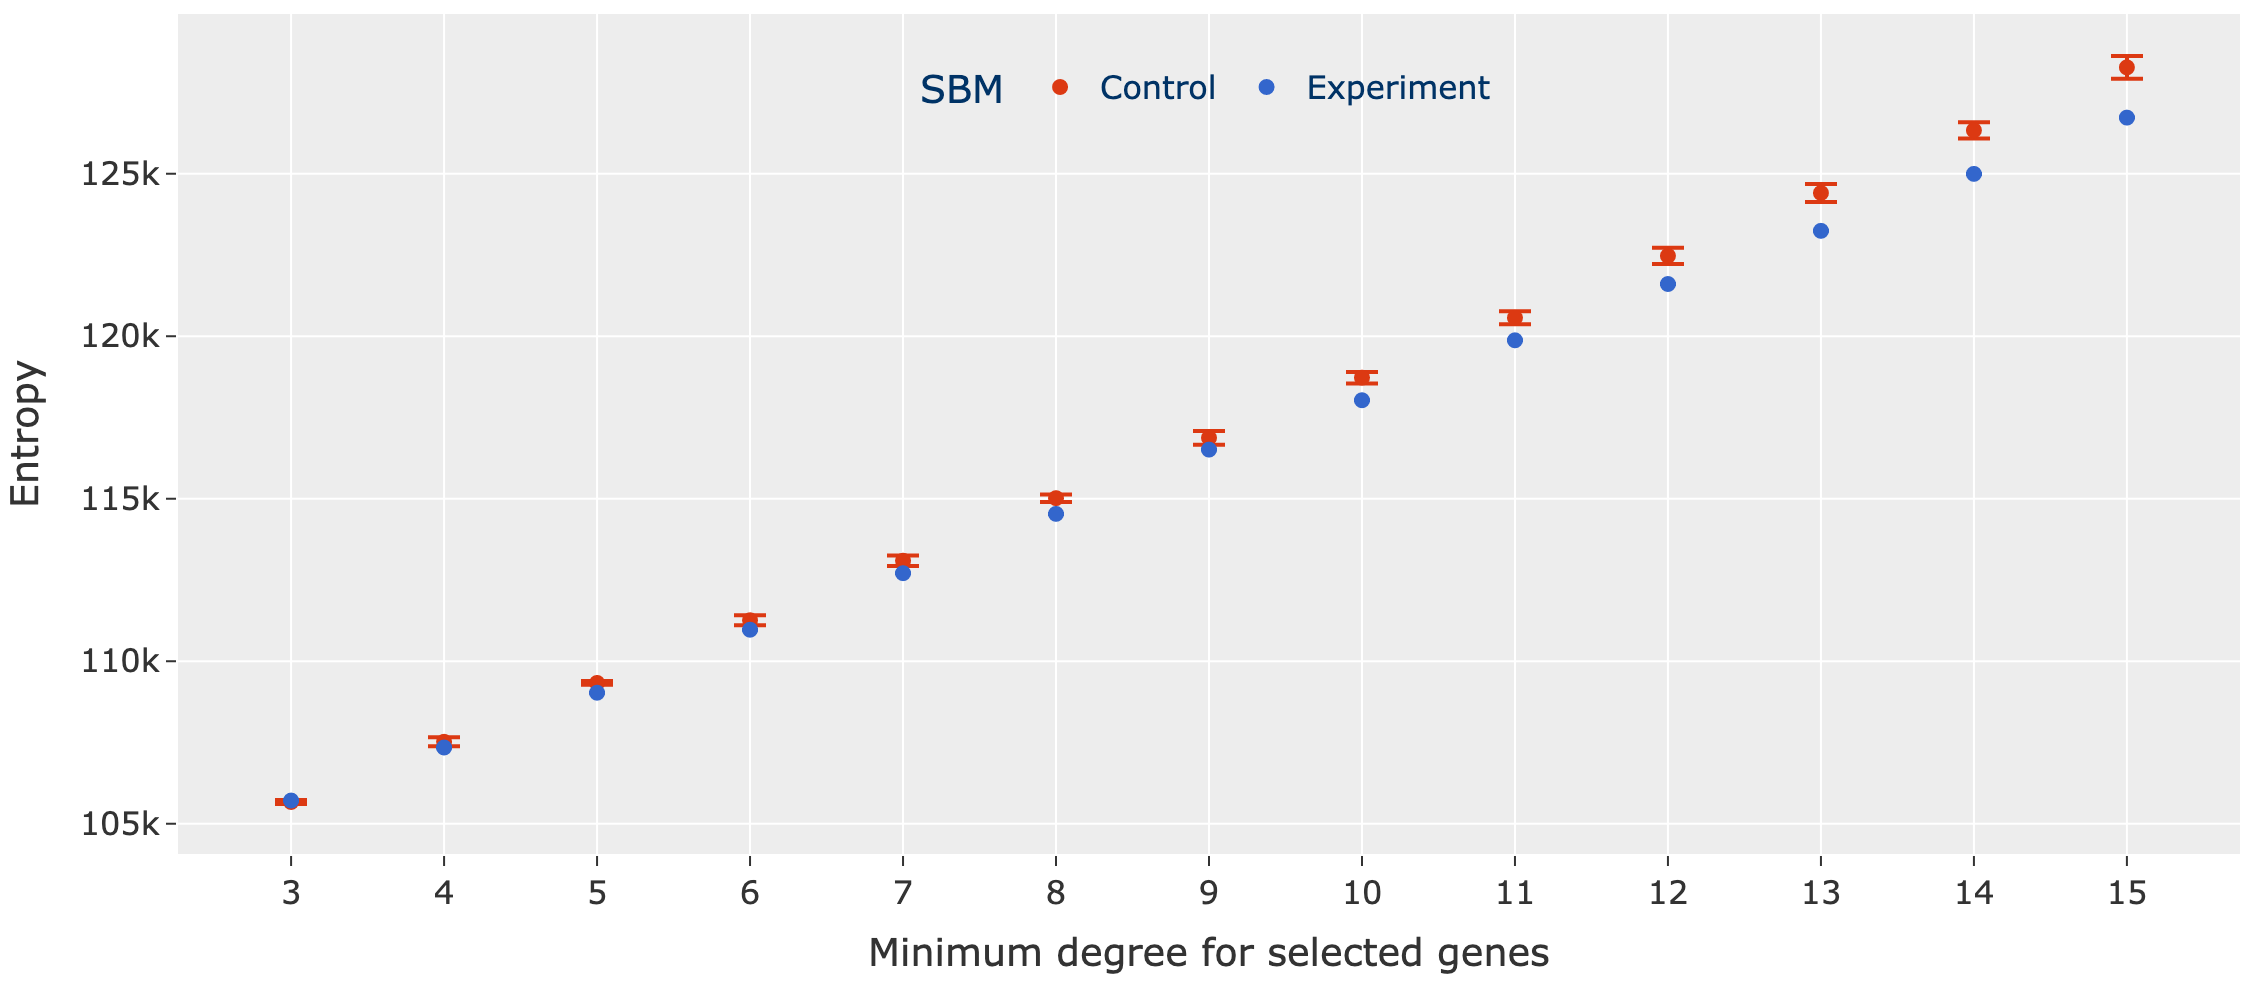
\includegraphics[width=\textwidth]{Sections/Network_I/Resources/selective_pruning/com_comp/sbm_ent_sel_prun.png}
        \caption{Stochastic Block Model}
        \label{fig:N_I:sbm_com_det_met}
    \end{subfigure}\hspace{\fill} 
    \begin{subfigure}[!t]{1.0\textwidth}
        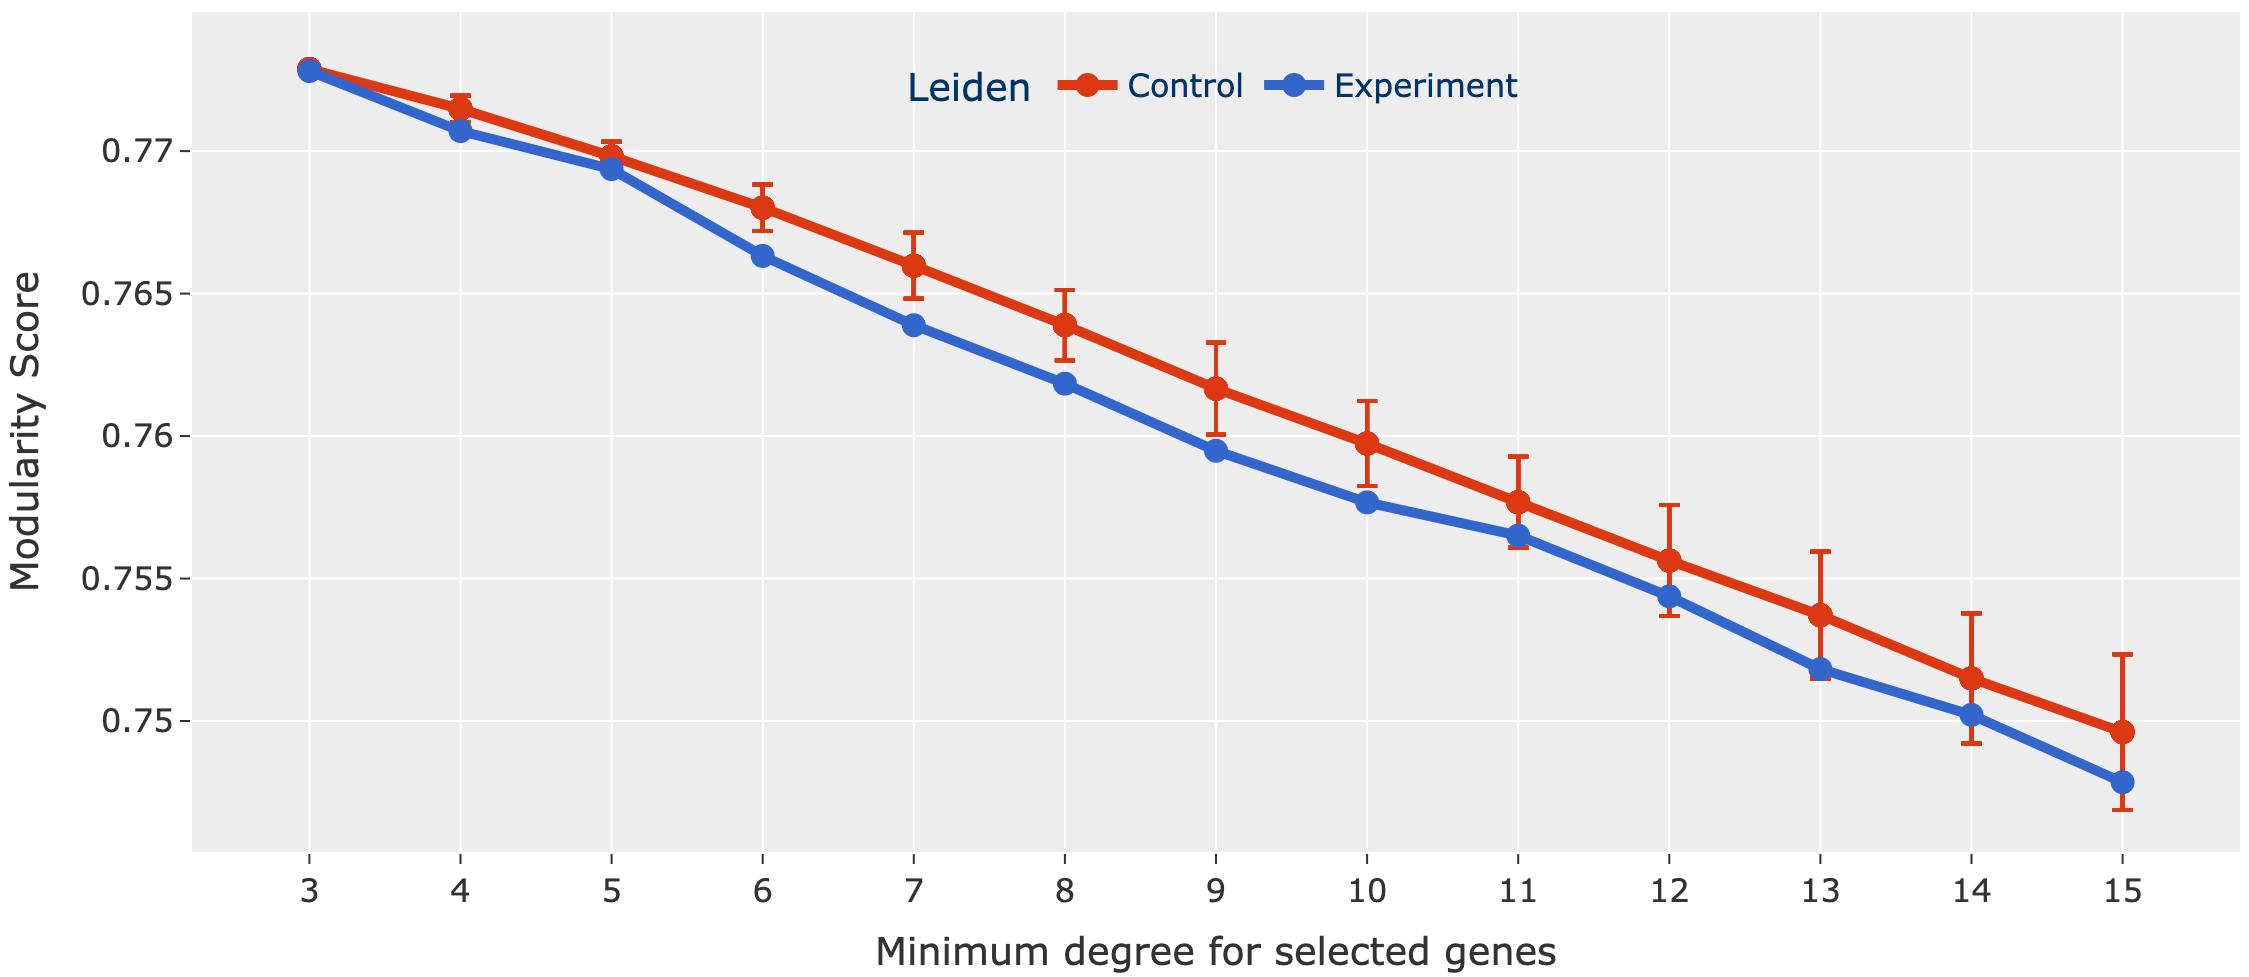
\includegraphics[width=\linewidth]{Sections/Network_I/Resources/selective_pruning/com_comp/leid_mod_sel_prun.png}
        \caption{Leiden}
        \label{fig:N_I:leid_com_det_met}
    \end{subfigure}
    \caption[Metrics comparison between Leiden and SBM]{Metrics comparison between Minimum Description Length (MDL) - entropy- in SBM (lower the better) and Modularity Maximisation in Leiden (higher the better). The error bars in the control is given by the standard deviations. As the minimum degree for the increases both community detection suffer a decrease in the performance. }
    \label{fig:N_I:com_det_met}
\end{figure}

% Introduce the figure
% \Cref{fig:N_I:comp_size_com_det} presents the effects of increasing the minimum degree to the community sizes for Leiden and SBM where the blue traces represent the experiments performed while the red the controls. 

% Comment com_size figure
Another major difference between Leiden and SBM is that the former finds consistently considerably more communities than the latter; see \cref{fig:N_I:comp_size_com_det}. It can be noticed that SBM has an upward trend proportional with the minimum degree of the nodes, this highlighted by the control experiments. In \cref{fig:N_I:comp_size_com_det}, Leiden appears to find the same number of clusters, but in the \cref{fig:ap:leid_com_size} from Appendix, where the Leiden traces are plot separately, it can be noticed that Leiden tends to finds less communities as the minimum degree is increased. 

\begin{figure}[!t]   
    \centering
    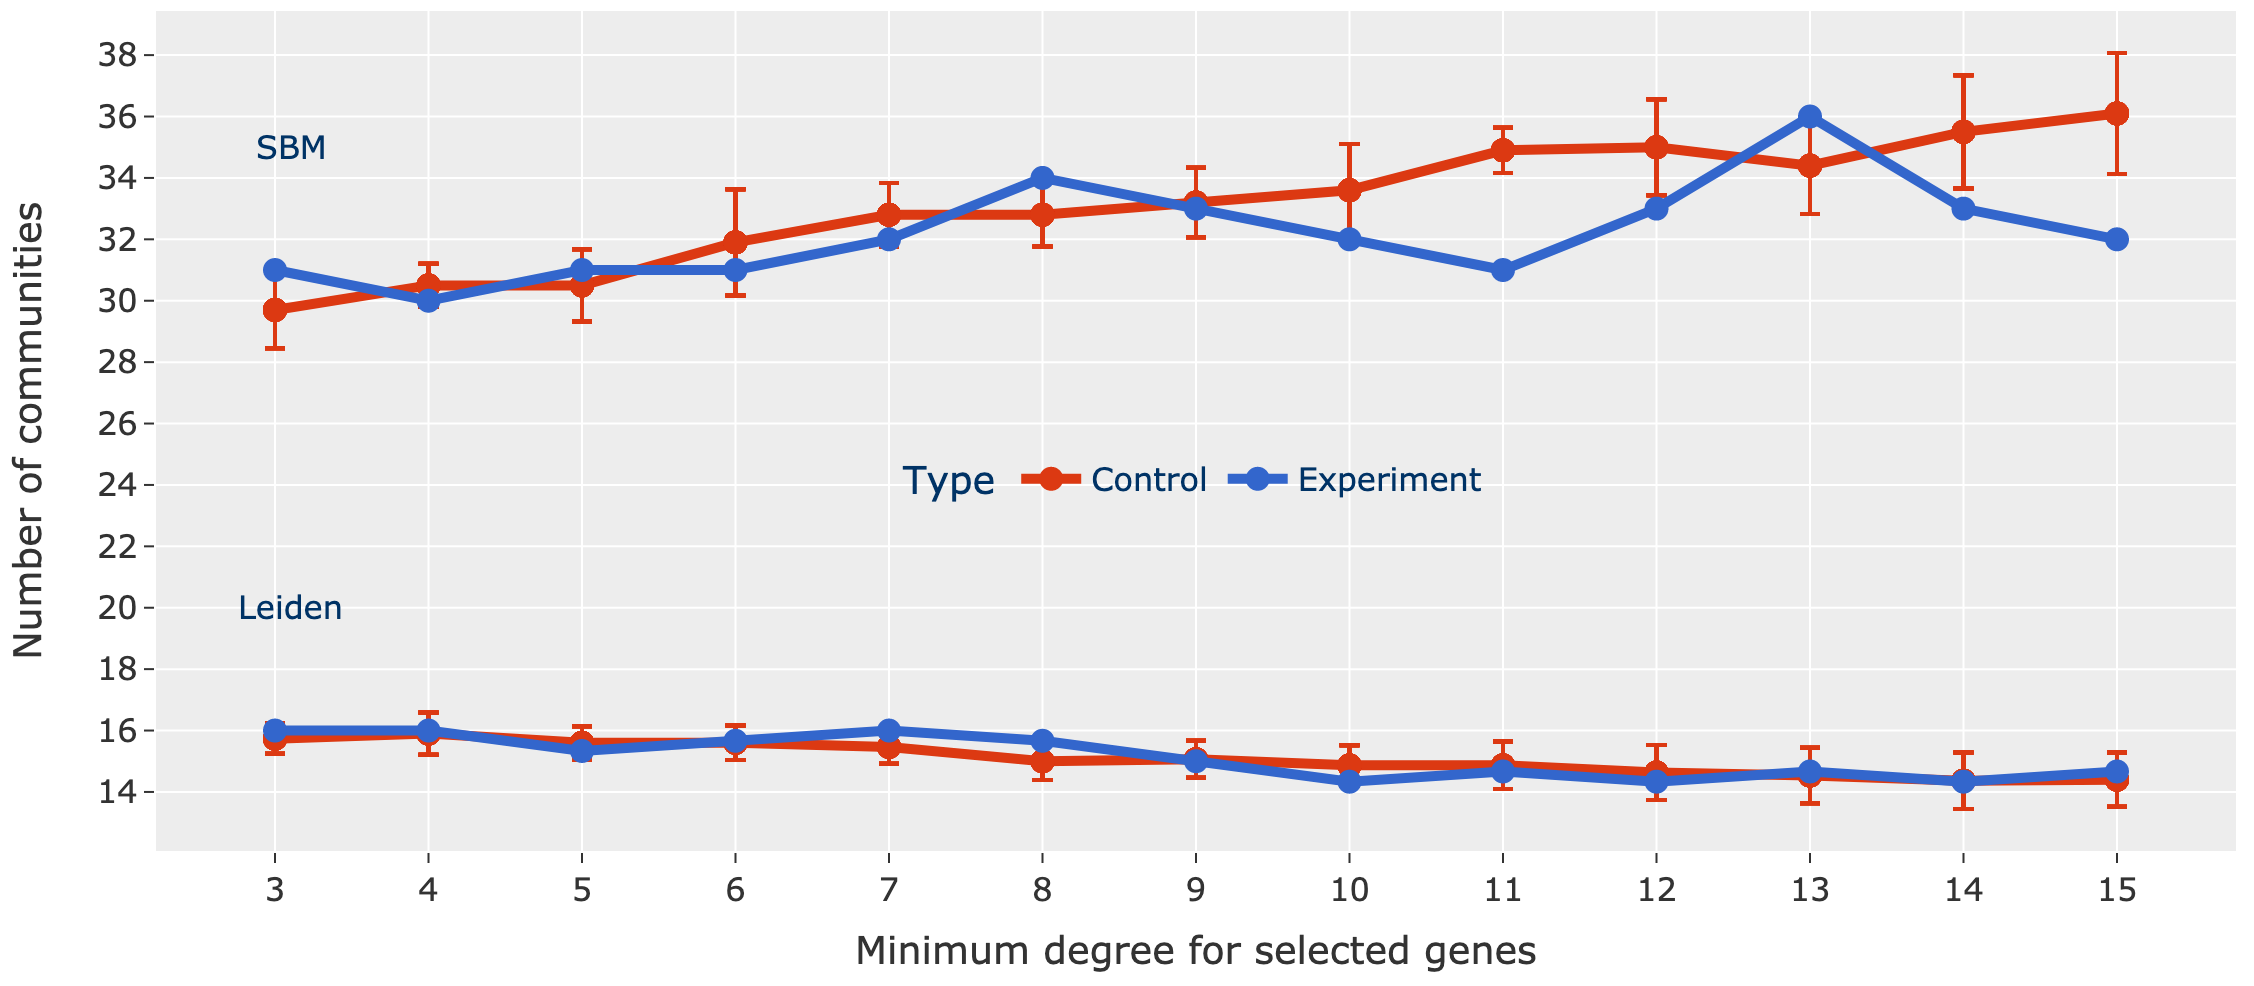
\includegraphics[width=1.0\textwidth,keepaspectratio]{Sections/Network_I/Resources/selective_pruning/com_comp/sbm_Leiden_combNum.png}
      \caption[Leiden vs SBM: Number of communities found]{Community size for Leiden and Stochastic Block Model. Blue lines are represented by the experiments run with biological TFs while the red ones are the controls, with non-TF genes. The error bars in the control is given by the standard deviations. The plot shows that SBM consistently find a large number of communities compared to Leiden. Another version of the plot where the trends of the two method are separated can be seen in \cref{fig:ap:leid_com_size} from Appendix.}
    \label{fig:N_I:comp_size_com_det}
\end{figure}

% Variance and that SBM is probabilistic
Growing the number of nodes also increases the variance in the number of communities found by the two methods. This be observed seen in \cref{fig:ap:com_size_comp} which shows the changes in the number of blocks across Leiden and SBM two separate figures. The plot indicates that SBM has a higher variance compared to Leiden when the number of edges are increased.
% However, due to the probabilistic nature of SBM it is possible to observe changes in the community members of the nodes. This helps feature might offer useful insights in the genes which are 'stable' and are important for a community.

% Summary
In summary, by increasing the minimum degree, both algorithms perform worse regardless of whether the prioritised genes are selected at random or have biological significance (i.e., TFs). SBM finds more communities compared to Leiden but has a higher variance. Given the probabilistic nature of SBM, additional useful information can be extracted from the network like gene membership. Importantly, from the work of \cite{Peixoto2023-mw} the SBM is more error proof to find patterns in noise; see community detection \cref{s:lit:comm_detect}. For this reason and the results in this section the stochastic model is the preferred method in this project.


% Analysing the TFs